\newpage

\section*{Anhang}
  \addcontentsline{toc}
    {section}
    {Anhang}



\subsection*{Elektronischer Anhang}\label{elect-anhang}
\addcontentsline{toc}
{subsection}
{Elektronischer Anhang}

Diese Dokumentation wurde zusammen mit einem elektronischen Anhang in Form einer ZIP-Datei abgegeben. Darin befinden sich der Simulator Programmiercode inklusive dessen Ergebnisse und die erstellten CAD Dateien.

\newpage
\subfile{parts/x-projektplanung}
\newpage

%%%%%%%%%%%%%%%%%% Aufgabenstellung

\subsection*{Originale Aufgabenstellung}\label{aufgabenstellung}
\addcontentsline{toc}
{subsection}
{Originale Aufgabenstellung}

Nachfolgend ist die originale Aufgabenstellung angehängt.

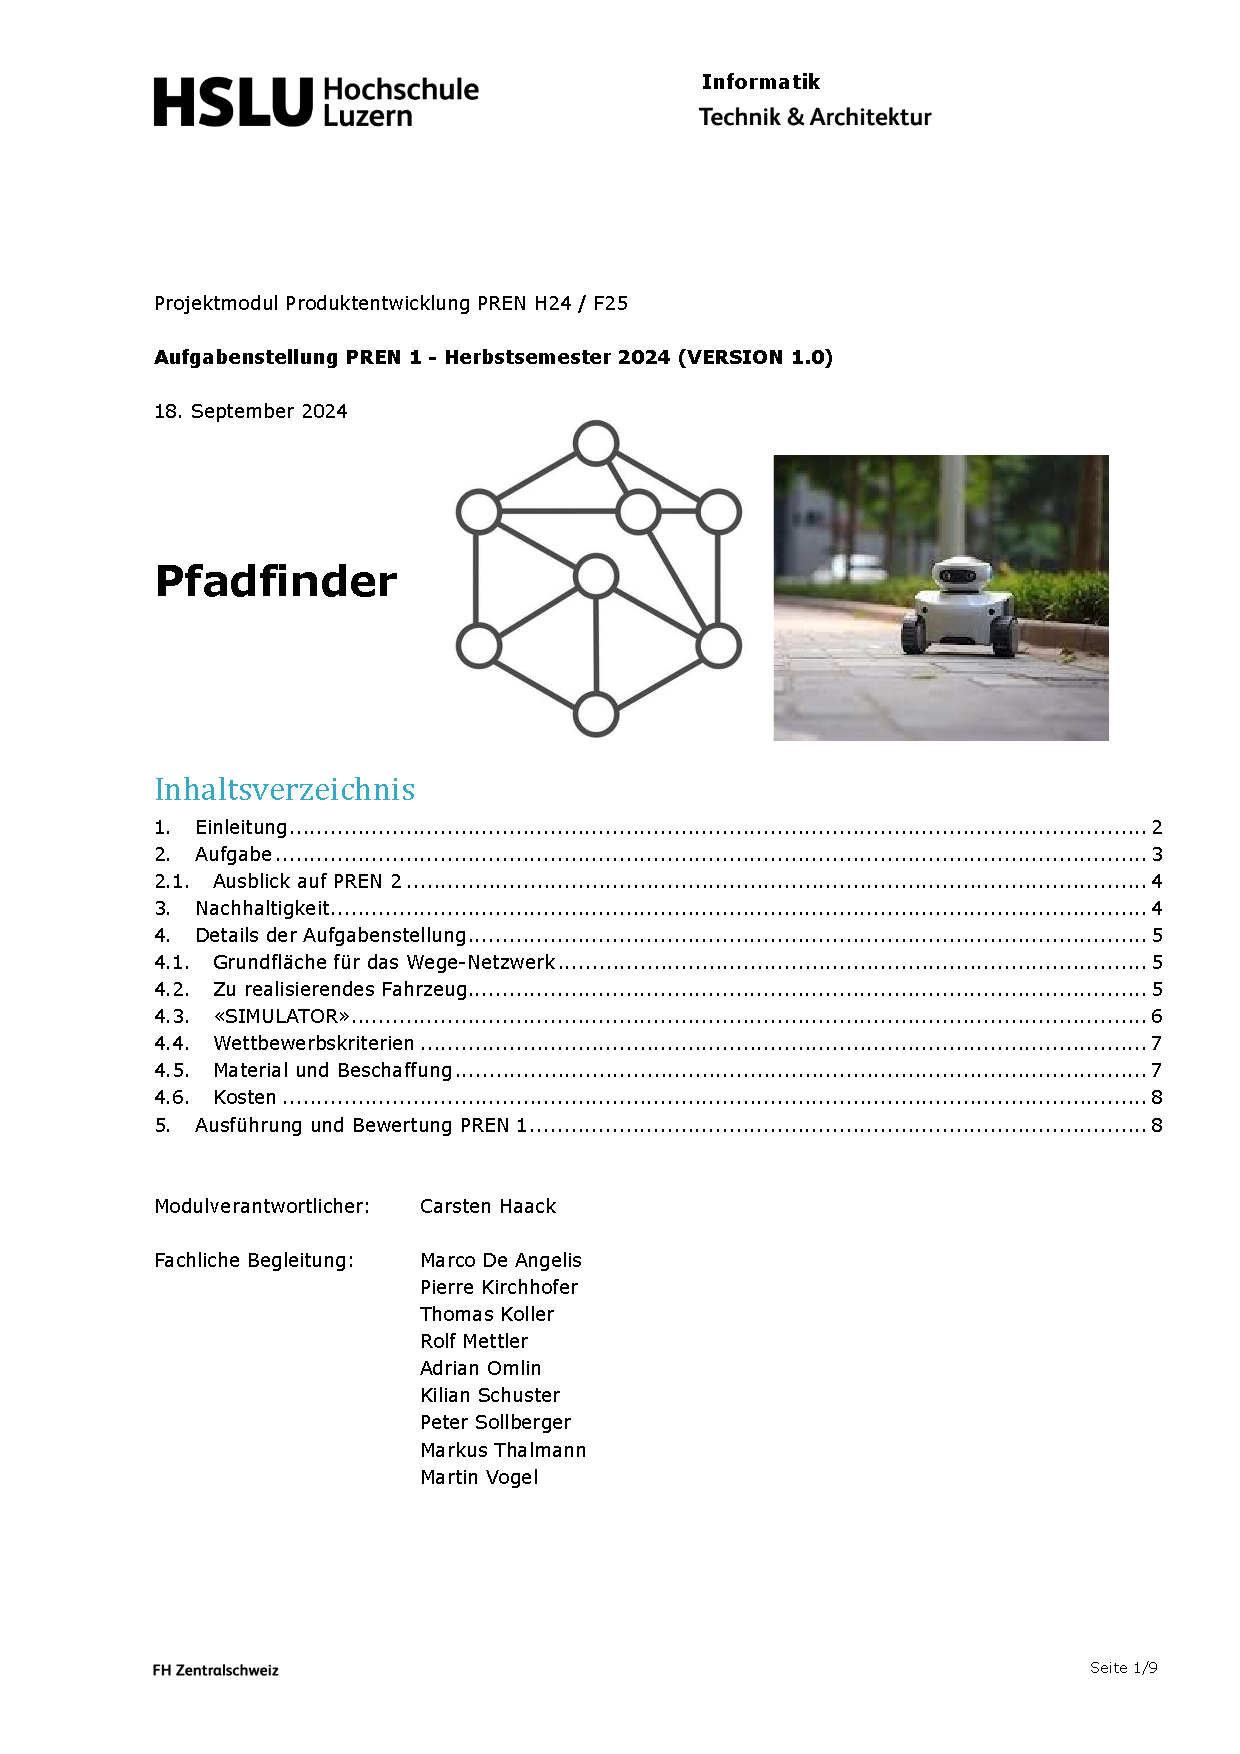
\includepdf[pages=-]{assets/projektmanagement/AufgabenstellungPREN1HS24.pdf}

%%%%%%%%%%%%%%% Anforderungsliste %%%%%%%%%%%%%%%%%%%%%%%%%

\subsection*{Anforderungsliste}\label{anforderungliste}
  \addcontentsline{toc}
    {subsection}
    {Anforderungsliste}
Die  Anforderungsliste ist ersichtlich in Tabellen \ref{table:anforderungsliste_page1} und \ref{table:anforderungsliste_page2}.

\begin{table}[H]
\centering
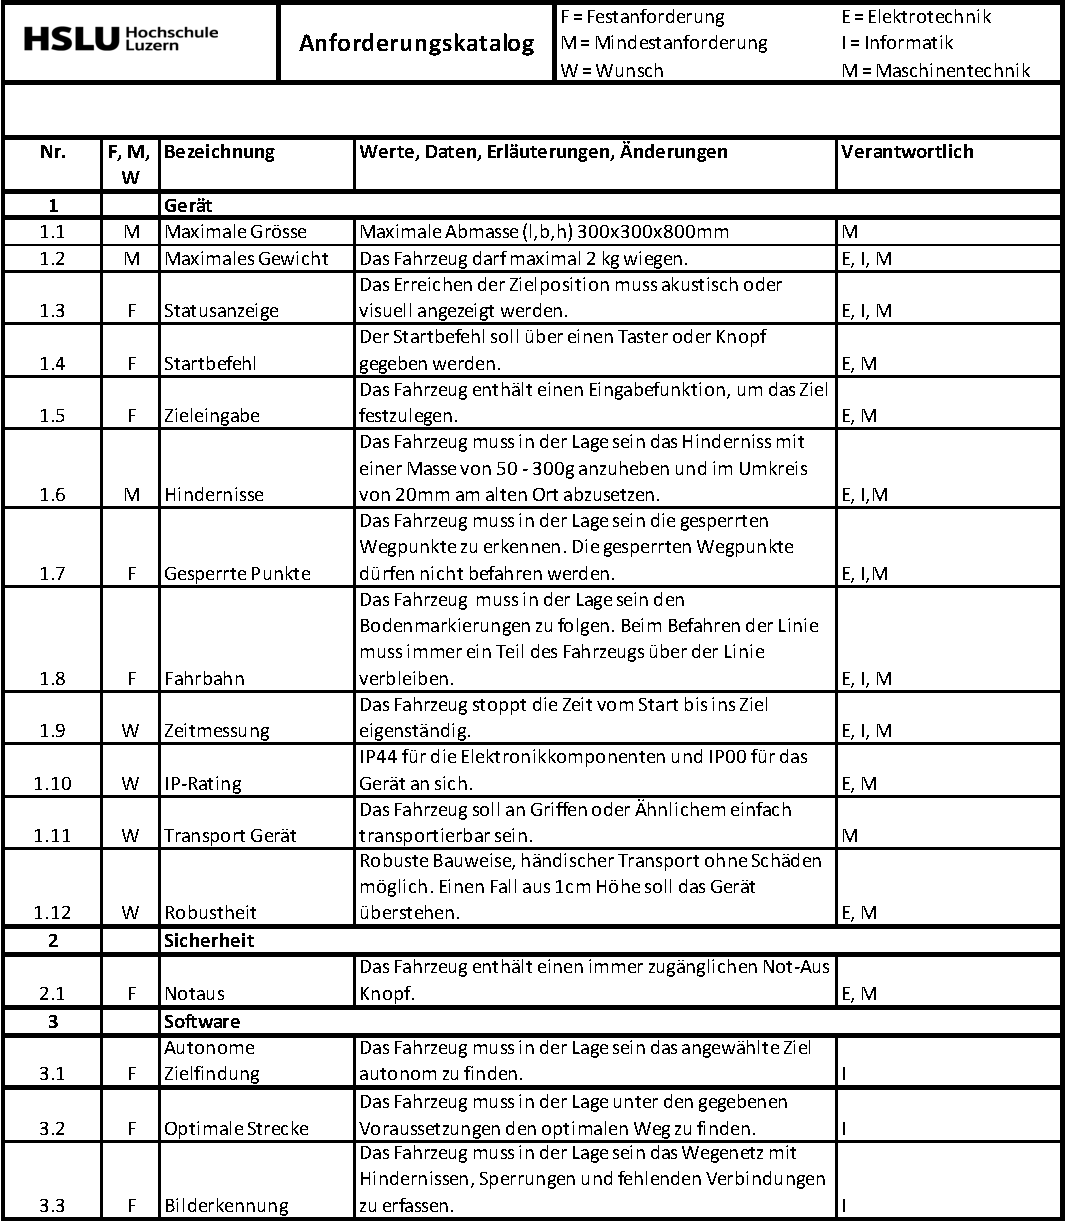
\includegraphics[width=\textwidth]{assets/projektmanagement/Anforderungsliste_V1.01_page1.pdf}
\caption{Anforderungsliste Teil 1}
\label{table:anforderungsliste_page1}
\end{table}
\newpage

\begin{table}[H]
\centering
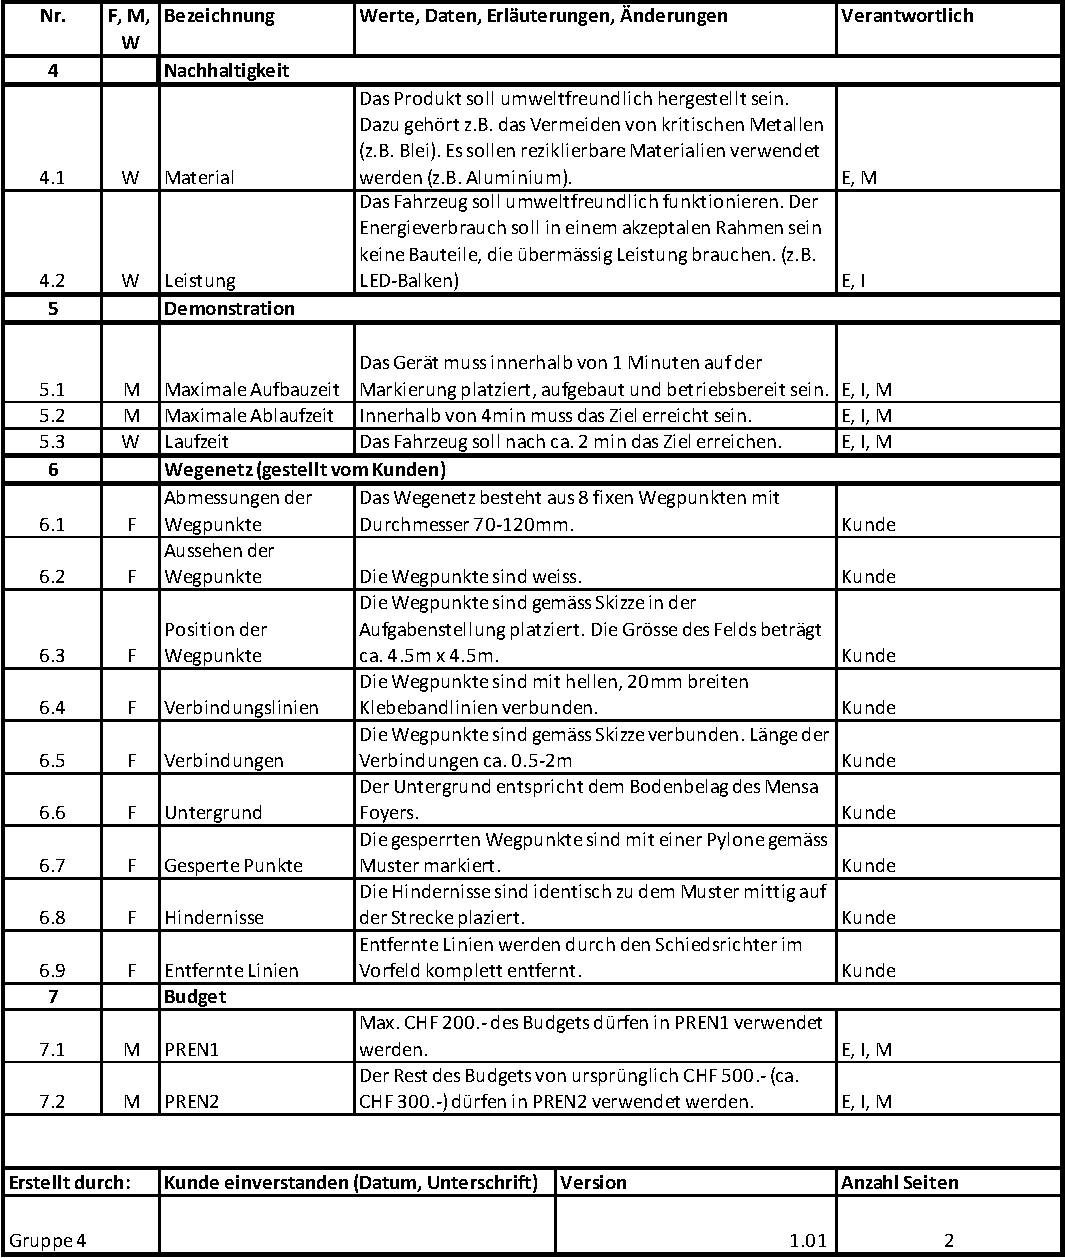
\includegraphics[width=\textwidth]{assets/projektmanagement/Anforderungsliste_V1.01_page2.pdf}
\caption{Anforderungsliste Teil 2}
\label{table:anforderungsliste_page2}
\end{table}
\newpage


%%%%%%%%%%%%%%%% Model Evaluation %%%%%%%%%%%%%%%%%%%%%%%%%5

\subsection*{YOLOv11 Model Evaluation}\label{model-evaluation}
  \addcontentsline{toc}
    {subsection}
    {YOLOv11 Model Evaluation}

Damit Pylonen, Barrieren und Knoten erkannt werden koennen, wird ein Model trainiert. Insgesamt wurden ueber 30 verschiedene YOLO Models trainiert. Viele davon wurden bereits in einem vorherigen Schritt aussortiert, da einige sehr offensichtlich schlechte Performance aufwiesen aufgrund davon, wie es die Objekte erkannt, beziehungsweise nicht erkannt hat. Auf der folgenden Seite ist eine Tabelle angehaent, in der die relevanten Models miteinander verglichen werden und das beste Model gewaehlt wurde.

Die Model Performance wird an folgenden Parametern gemessen:\cite{model-performance}

\begin{itemize}
    \item Confusion Matrix: Zeigt was das Model vorhergesagt hat und was tatsaechlich zu sehen war. Je 'diagonaler' die Matrix, desto besser.
    \item F1-Confidence: Zeigt die Balance zwischen Confidence (Wahrscheinlichkeit, dass Vorrausgesagtes stimmt) und F1 Score (Harmonischer Durchschnitt von Recall und Precision). Je hoeher der F1 Wert, desto besser.
    \item Precision-Confidence: Zeigt die Balance zwischen Precision (Anteil von 'True Positives'; wenn Model sagt, es gibt einen Knoten, wie akkurat ist diese Deutung?) und Confidence. Je tiefer die Confidence, desto besser, da dadurch der hoechste Praezisionswert bereits bei einer tieferen Confidence erreicht wird.
    \item Precision-Recall: Zeigt die Balance zwischen Precision und Recall (Faehigkeit, alle Instanzen zu erkennen). Je hoeher die Precision, desto besser.
    \item Recall-Confidence: Zeigt die Balance zwischen Recall und Confidence. Je hoeher der Recall, desto besser.
    \item Lernverlauf: Zeigt inwiefern der Verlust (Unterschied zwischen Vorhergsagtem und Realitaet) sinkt bei den Trainingsdaten und den Validationsdaten. Beginnt der Verlust bei der Validation zu steigen, deutet dies auf Overfitting hin\footnote{https://developers.google.com/machine-learning/crash-course/overfitting/overfitting}. Sollte exponentiell sinken. Zeigt, wie das Model and Wissen gewinnt. Sollte expontentiell steigen.
\end{itemize}


Der Vergleich zwischen mehreren potentiellen Modellen ist in folgendem Dokument ersichtlich. Zwei Modelle wurden jeweils verglichen aufgrund von mehreren Werten. Ist der jeweilige Wert des einen Models besser, wird diese Zelle gruen eingefaerbt.

Es wurde untersucht, ob das Modell bessere Ergebnisse bringt, wenn die beiden Barrieren pro Farbe in einzelnen Klassen aufgeteilt werden oder nicht und verschiedene Augmentationen wurden verglichen. Augmentationen werden auf die Trainingsbilder angewandt, damit diese diverser sind und zum einen mehr der Realitaet entsprechen und auch um mehr Trainingsmaterial zu haben. Ebenfalls wurde experimentiert mit unterschiedlichen Groessen der Bilder. 

\includepdf[pages=-]{assets/IT/testing/yolo/ModelComparison.pdf}


%%%%%%%%%%%%%%%%%%%%%%%%%%%% Unittests %%%%%%%%%%%%%%%%%%%%%%%%%%%

\subsection*{Navigation automatisierte Unittests}\label{nav-unittests}
  \addcontentsline{toc}
    {subsection}
    {Navigation automatisierte Unittests}

TODO ADD FOR EACH MODULE THAT WE HAVE, SHOW IMAGES WHERE WE USE IMAGES



%%%%%%%%%%%%%%%%%%%%%%% protocol opencv calibration %%%%%%%%%%%%%%%%%%%%%%%%

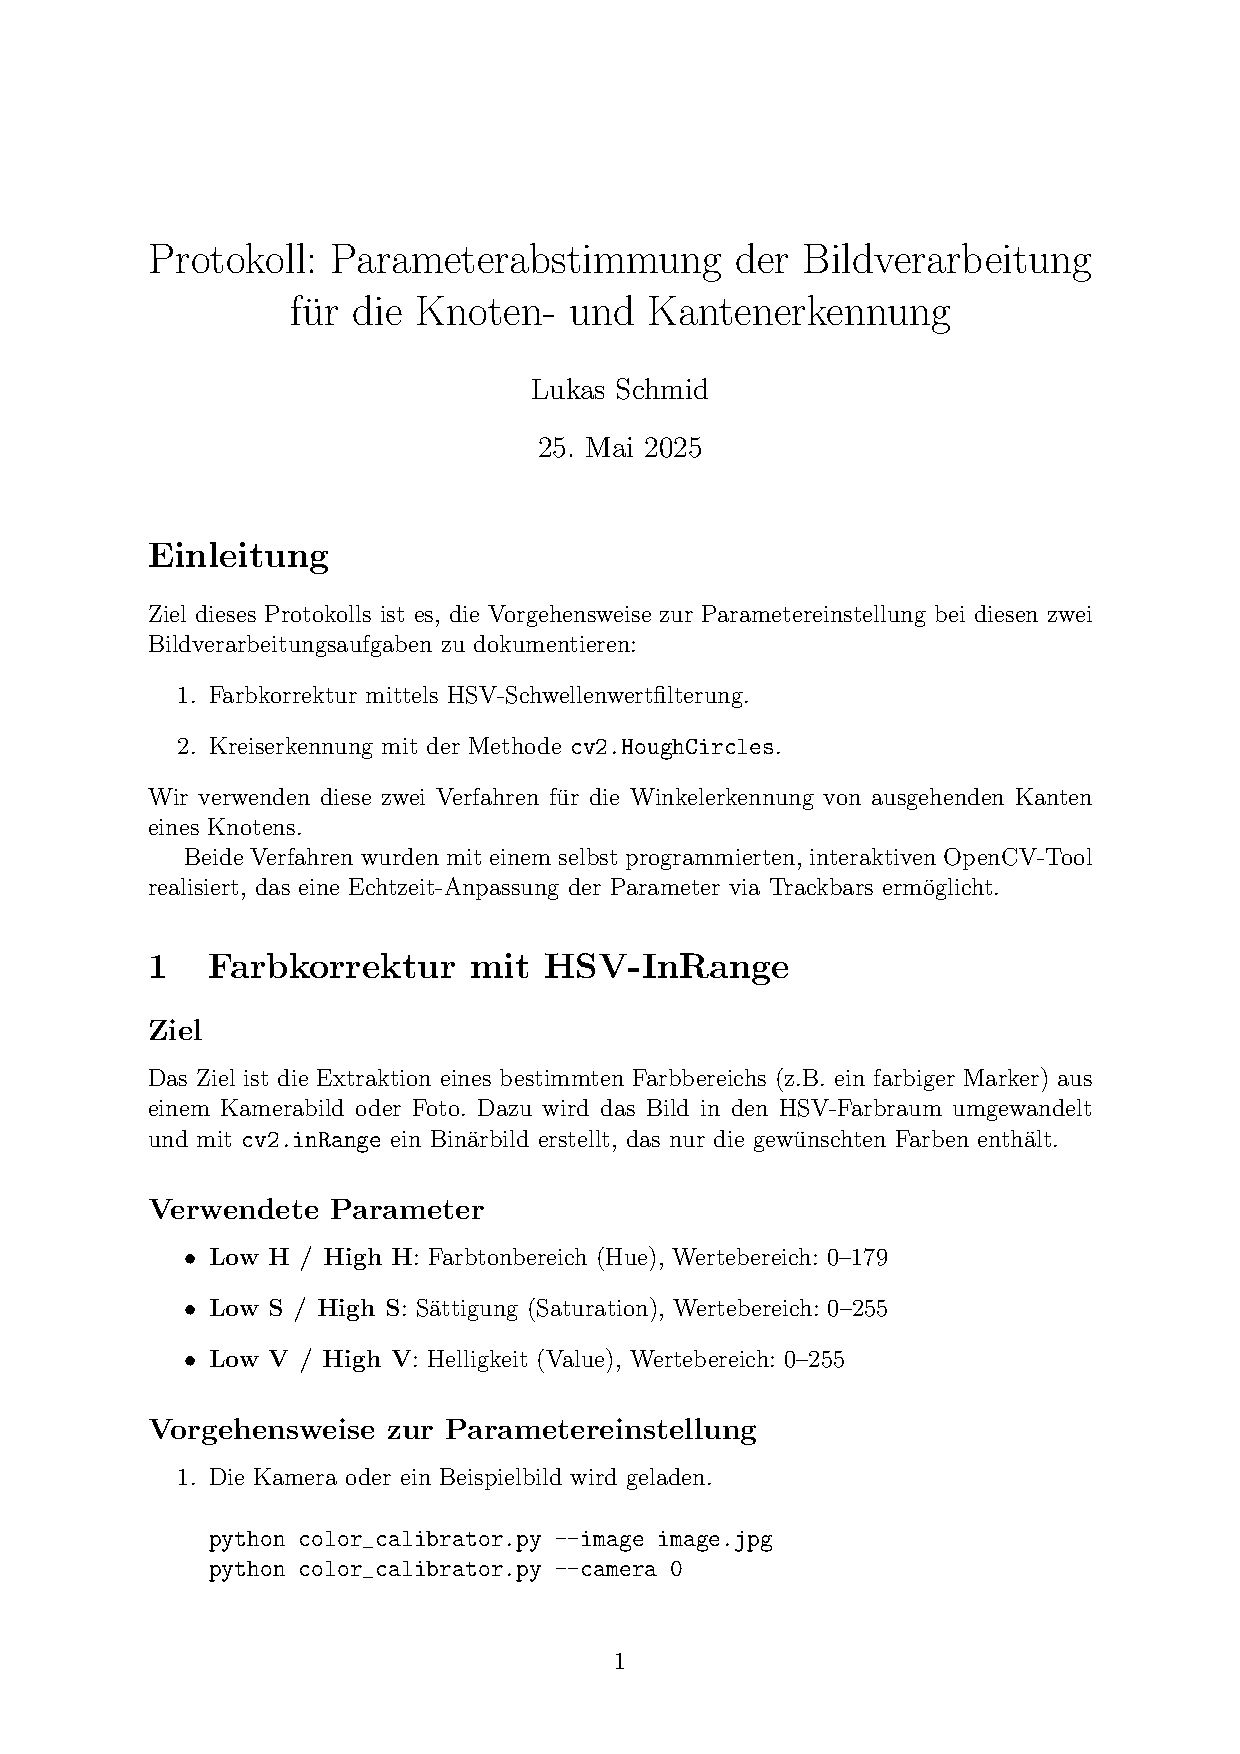
\includepdf[pages=-]{assets/IT/testing/protocol_opencv_calibration.pdf}


%%%%%%%%%%%%%%%%%%%%%%% testprocotol static node and edge detection %%%%%%%%%%%%%%%%%%%%%%%%

\includepdf[pages=-]{assets/IT/testing/testprotocol_static_node_edge_detection.pdf}